%\begin{figure}[t]
%
%   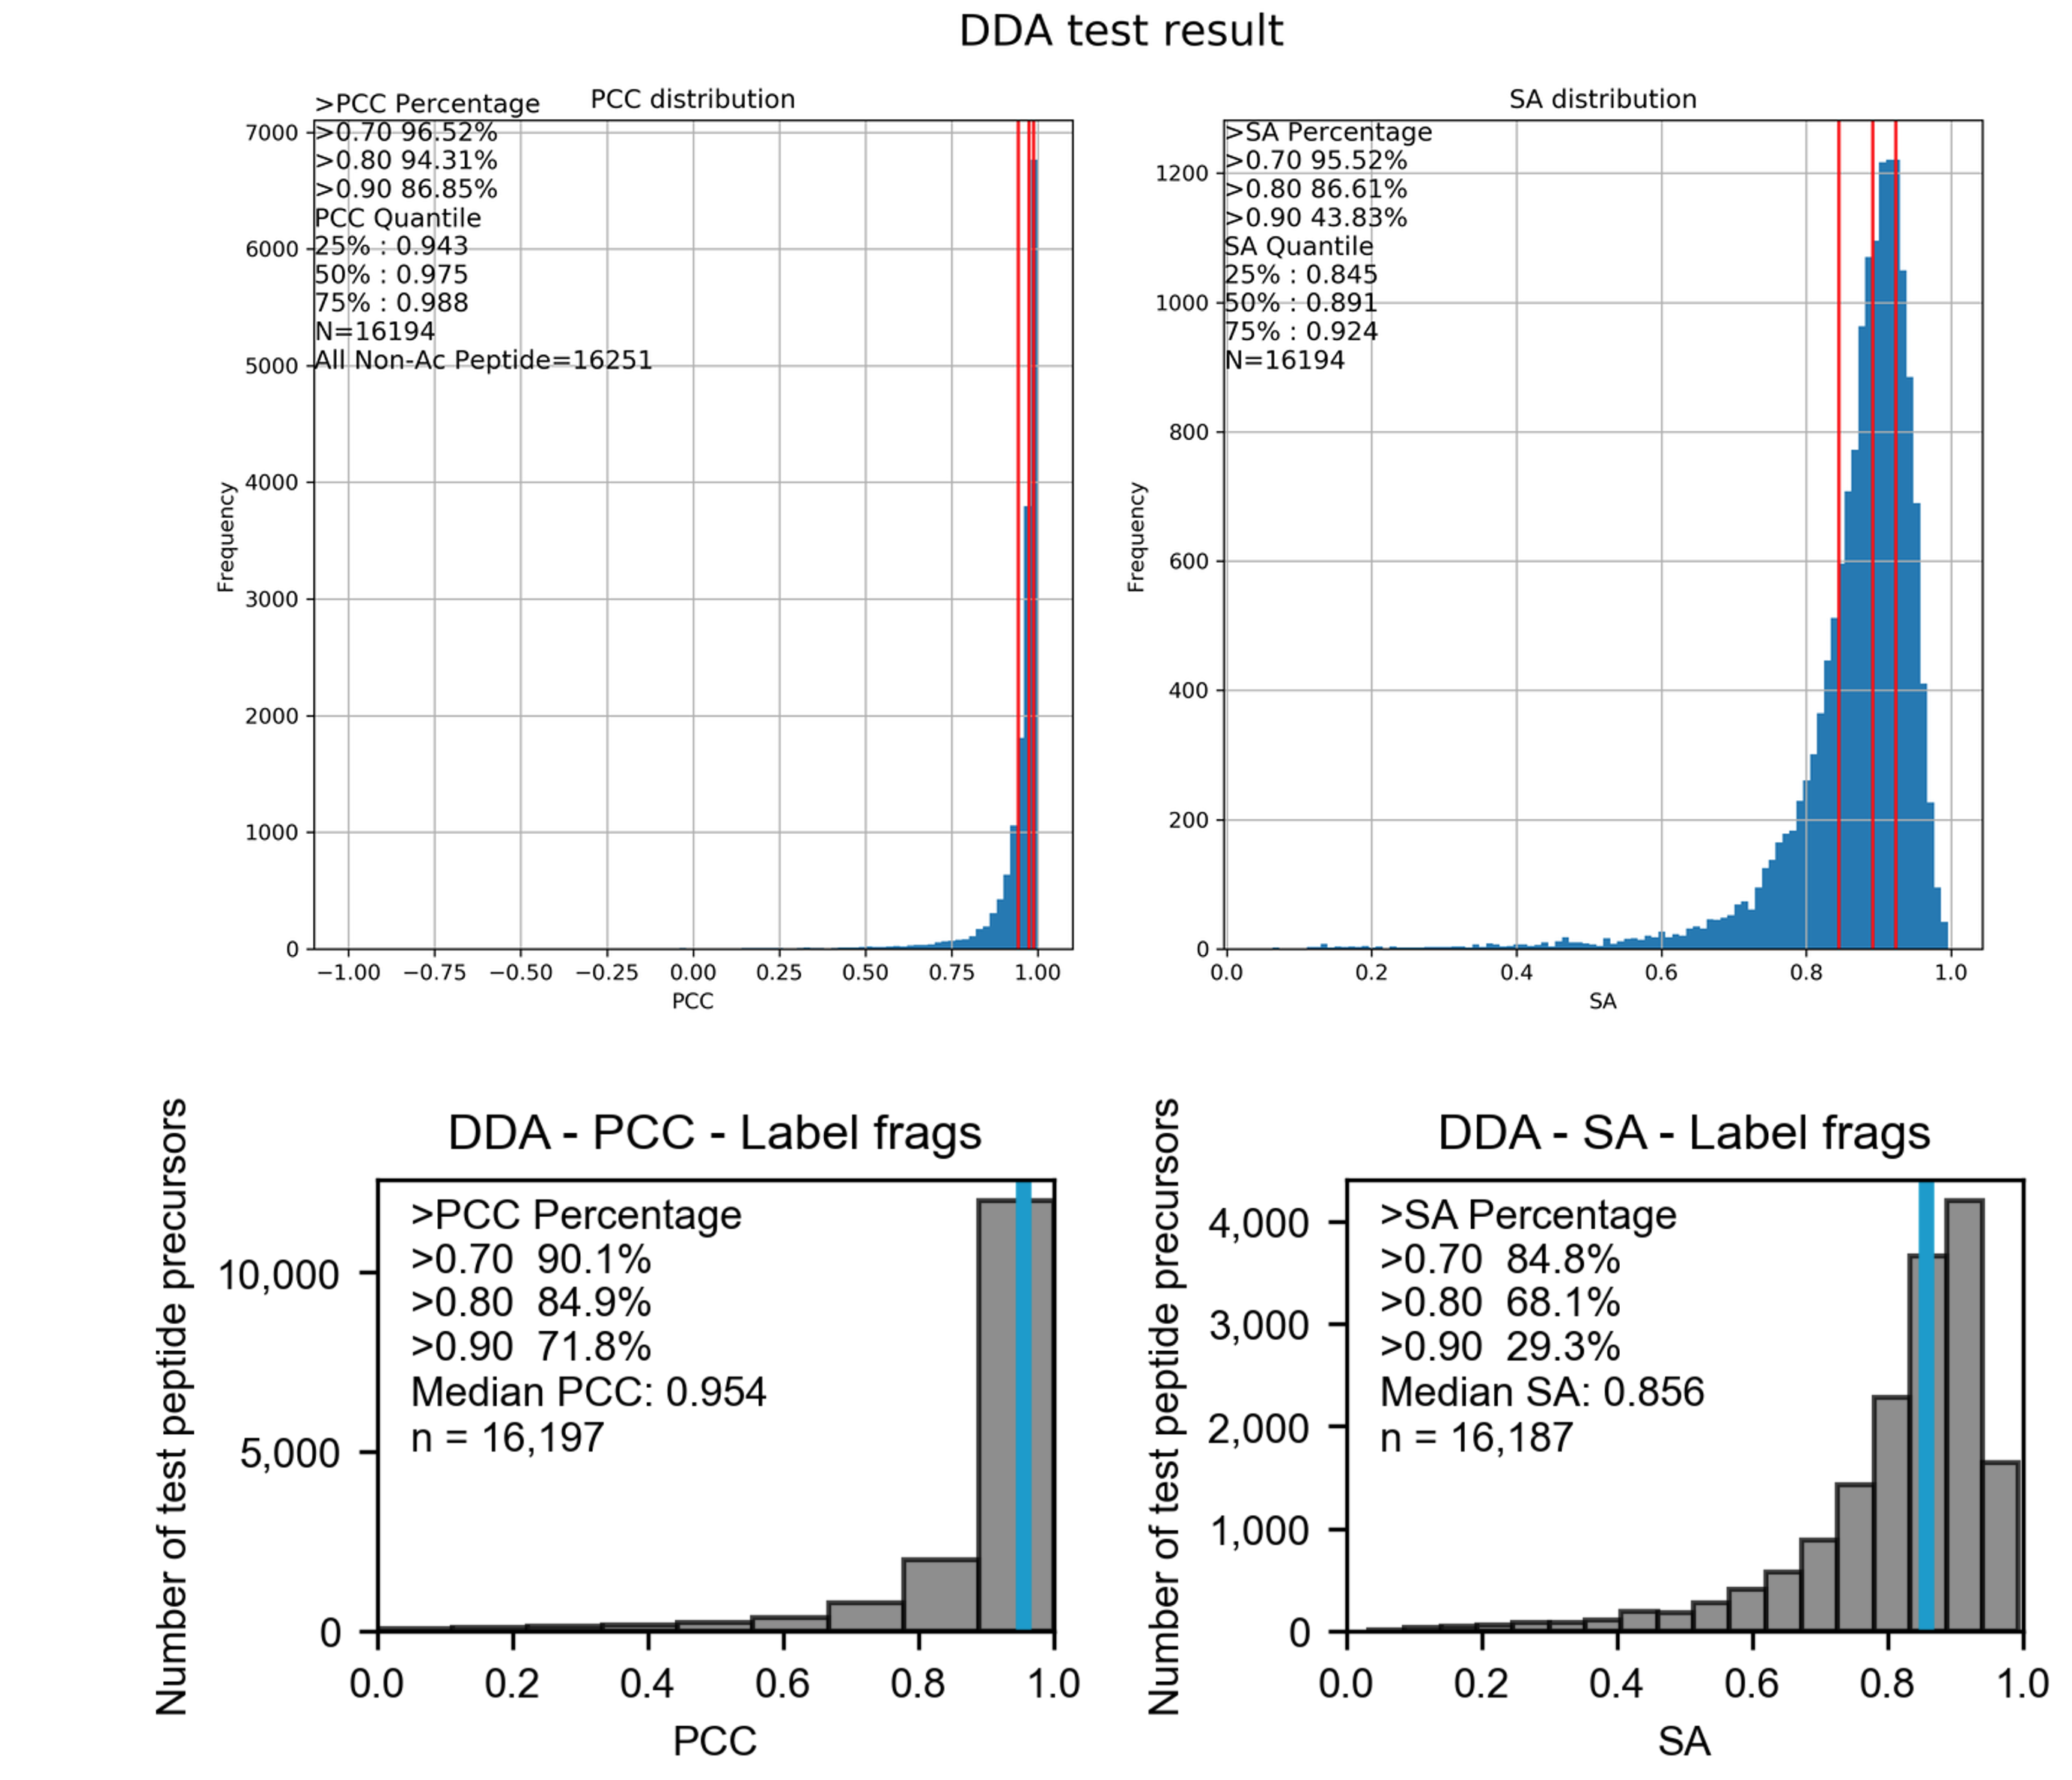
\includegraphics[width=3.0in]{DDA}
%
%   \caption{Visualization of performance of DDA dataset. The above is ours and the below is pdeep2}
%\label{fig:DDA}
%\end{figure}
%
%
%\begin{figure}[t]
%
%   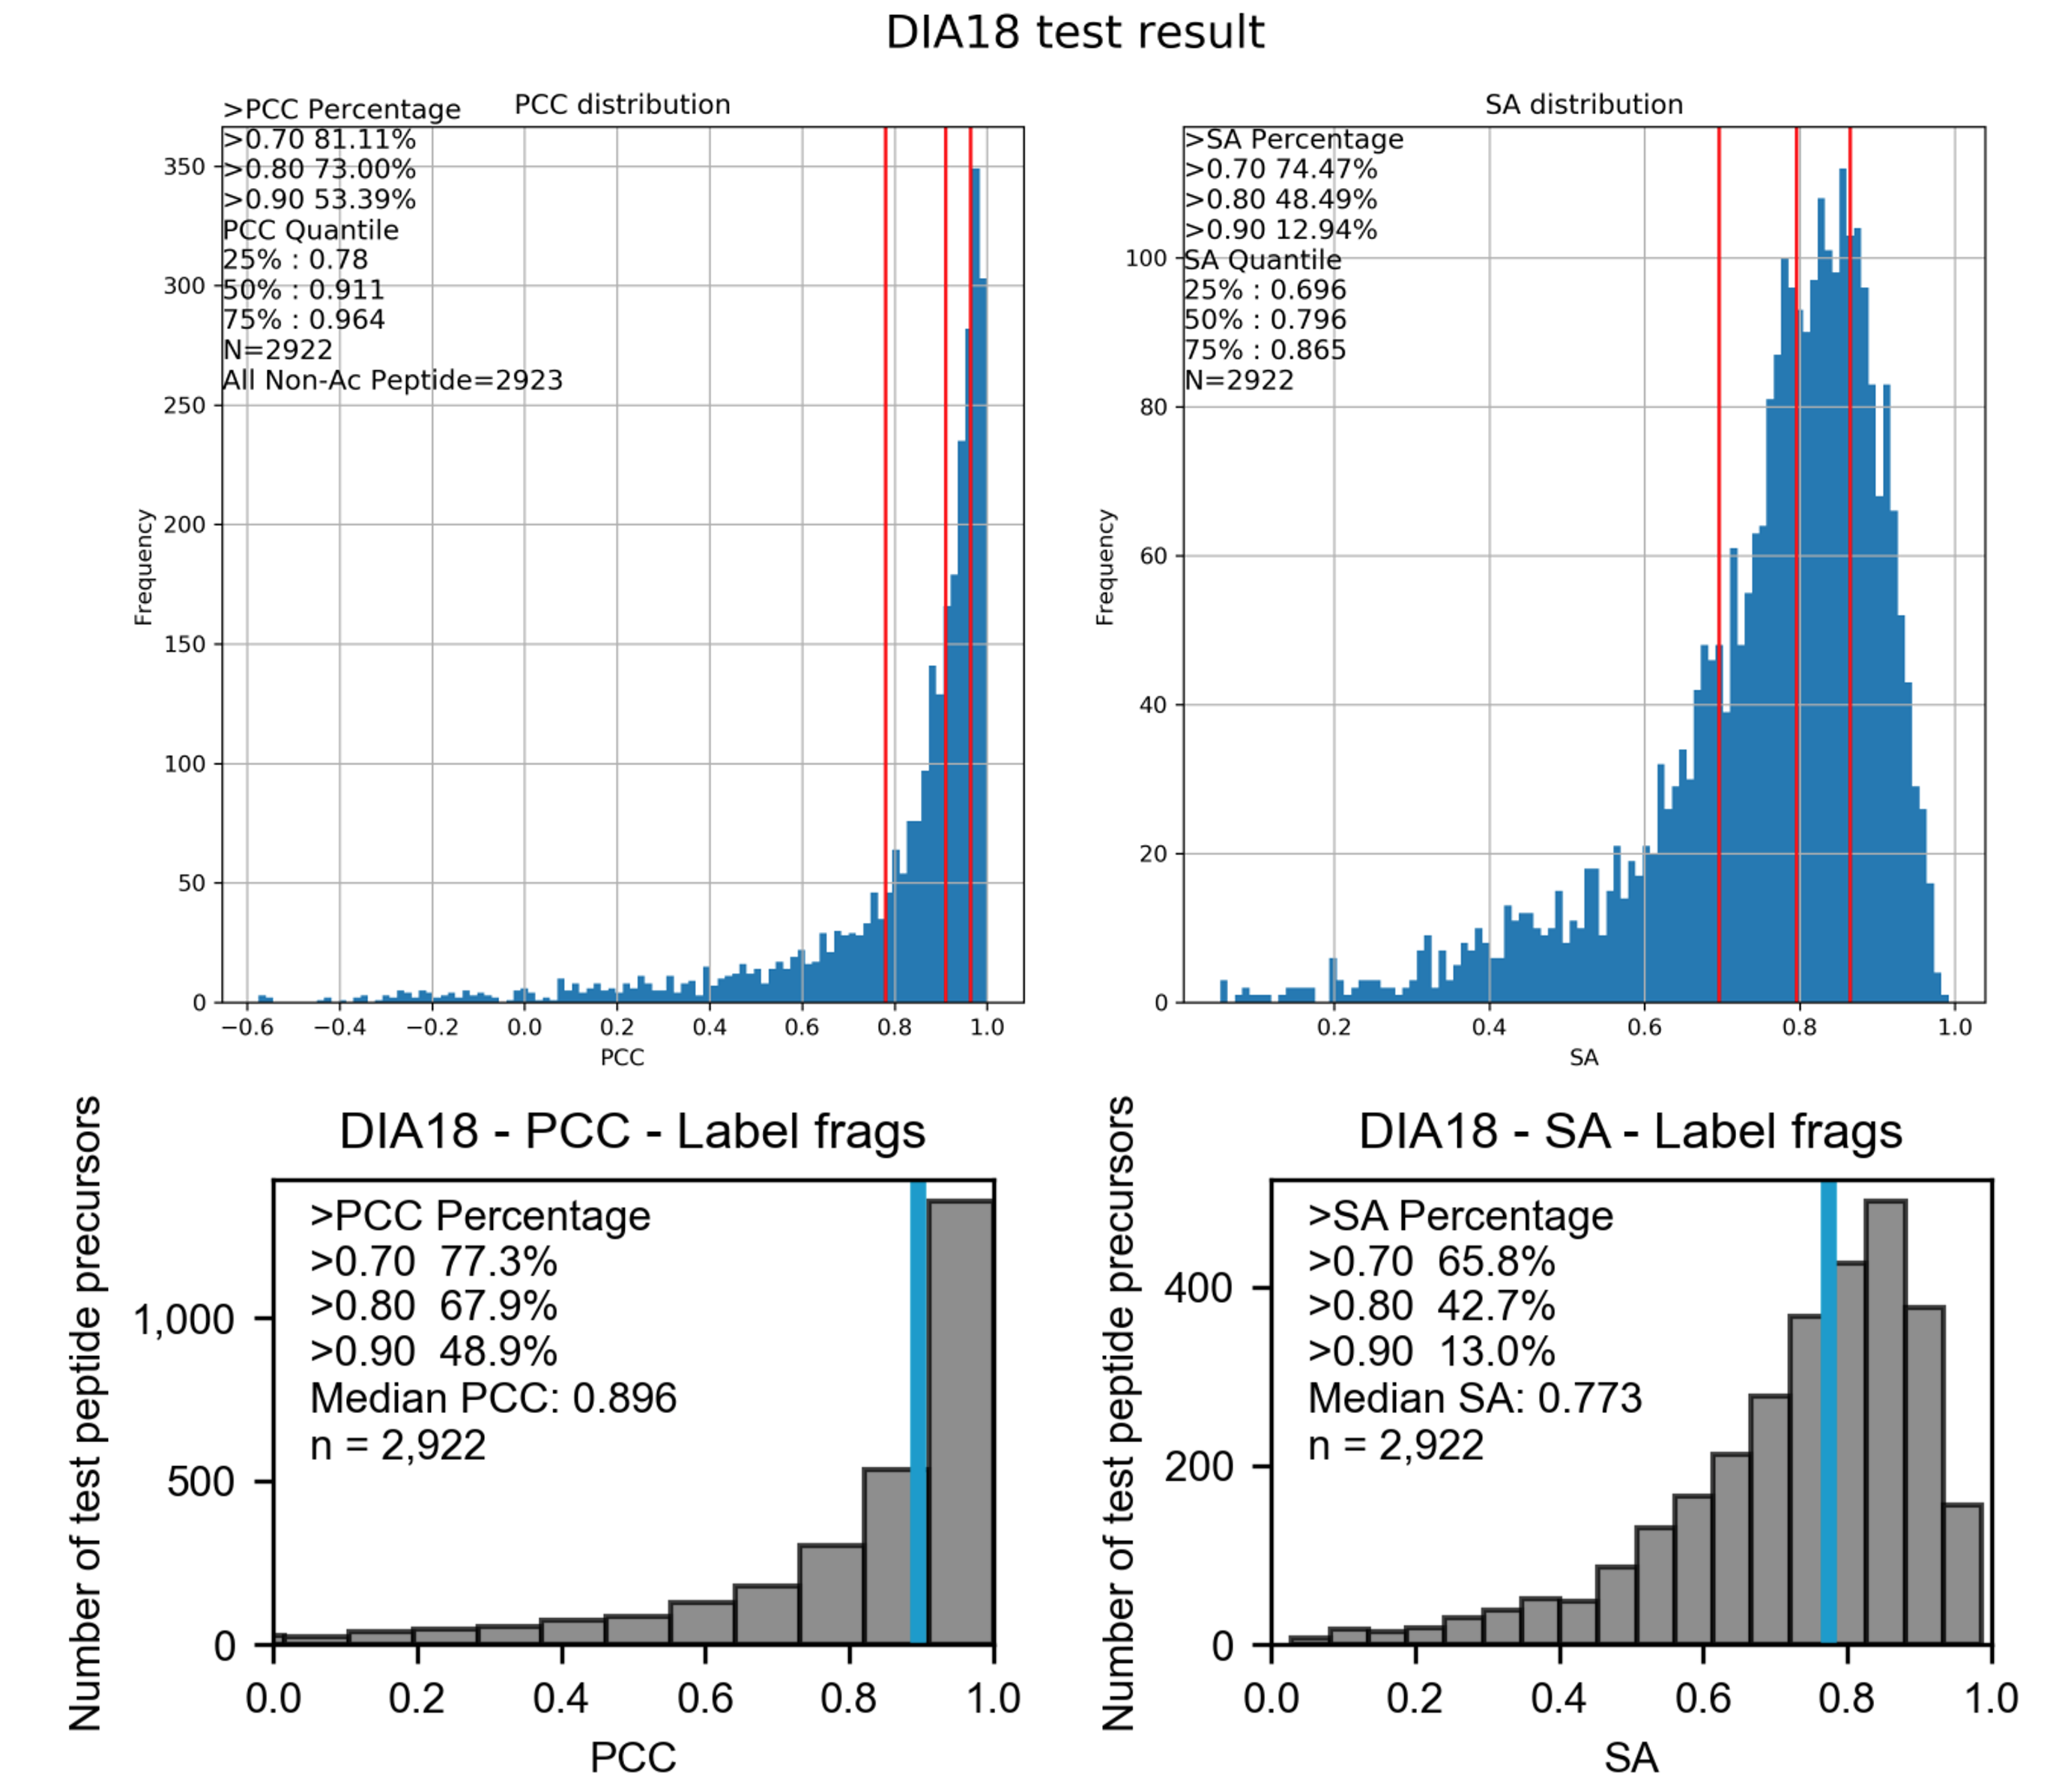
\includegraphics[width=3.0in]{DIA18}
%
%   \caption{Visualization of DIA18 dataset. The above is ours and the below is pdeep2}
%\label{fig:DIA18}
%\end{figure}
%
%
%\begin{figure}[t]
%
%   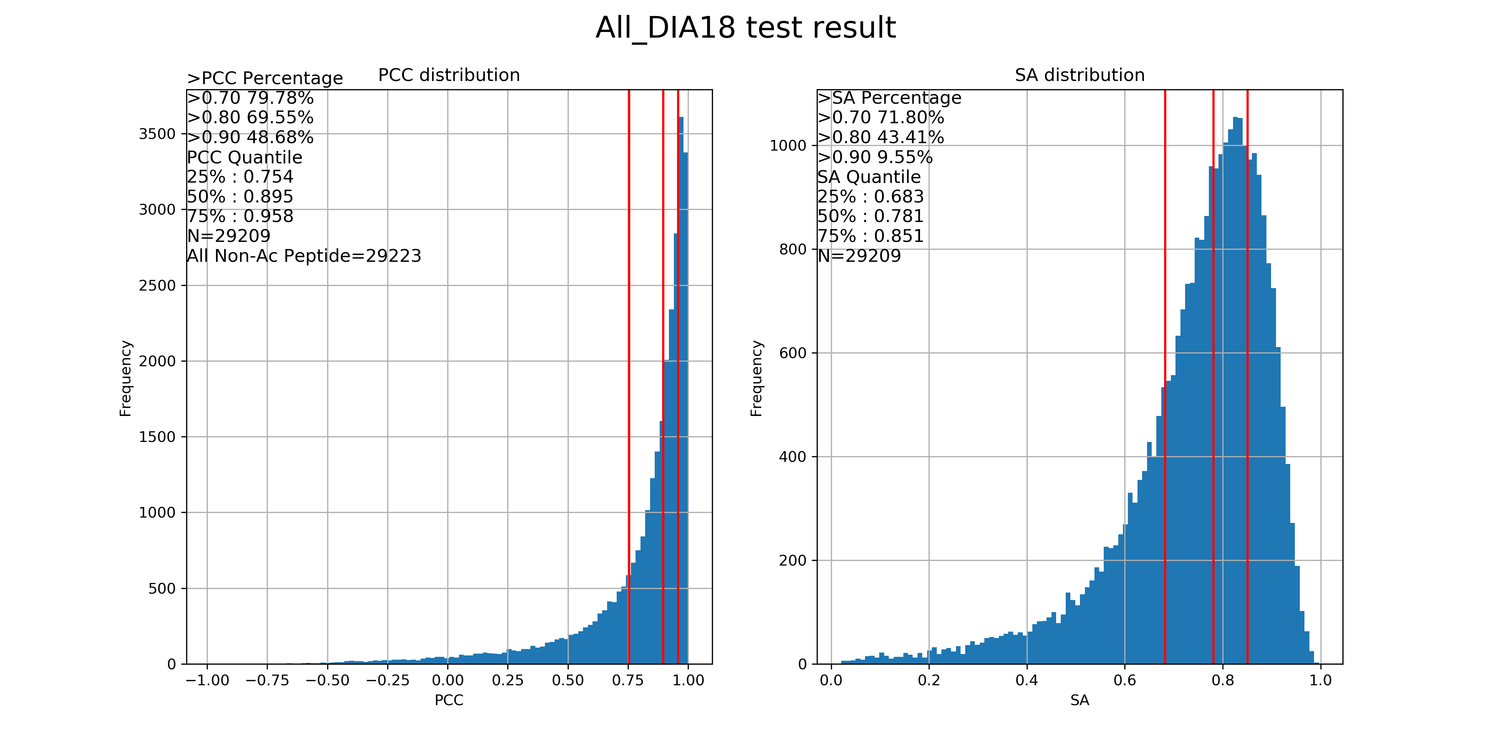
\includegraphics[width=3.5in]{DIA_direct_test}
%
%   \caption{Direct test on DIA18 dataset.}
%\label{fig:DIA18_direct}
%\end{figure}
%

\begin{table}
    \begin{center}
    \begin{tabularx}{\columnwidth}{|m{0.3\columnwidth}|Y|Y|}
    \hline
    data description & no. of peptides & no. of spectra\\
    \hline
    HumanPhosDB~\cite{lawrence2016plug} & 204,558 & -\\
    Jeff~\cite{liu2018vivo} & 67,552 & 89,437\\
    VeroE6~\cite{bouhaddou2020global} & 43,405  & 54,004\\
    R2P2~\cite{leutert2019r2} & 35,808 & 43,312\\
    U2OS-DIA~\cite{wang2020naguider} & 48,327 & 58,843\\
    RPE1-DIA~\cite{bekker2020rapid} & 33,576 & 39,977\\
    RPE1-DDA~\cite{bekker2020rapid} & 129,109 & 165,719\\
    \hline
    \end{tabularx}
    \end{center}
    \caption{Retention time datasets}
    \label{table:Datasets}
    \end{table}
 
    \begin{table}
       \begin{center}
      \resizebox{\columnwidth}{!}$ where the lower is the better, and the right is PCC where the higher is the better.}
       \label{table:Jeff}
       \end{table}
 
 \begin{table}
    \begin{center}
    \begin{tabular}{|l|c|c|}
    \hline
    Model & Median PCC & Median SA \\
    \hline\hline
    pdeep2 & 0.954 & 0.856 \\
    DeepPhospho$\star$ & 0.975 & 0.891 \\
    \hline
    \end{tabular}
    \end{center}
    \caption{DDA Dataset results.Ours is better.}
    \label{table:DDA}
    \end{table}
 
 \begin{table}
    \begin{center}
    \begin{tabular}{|l|c|c|}
    \hline
    Model & Median PCC & Median SA \\
    \hline\hline
    pdeep2 & 0.896 & 0.773 \\
    DeepPhospho$\star$ & 0.911 & 0.796 \\
    \hline
    \end{tabular}
    \end{center}
    \caption{DIA18 Dataset results.Ours is better.}
    \label{table:DIA18}
 \end{table}
 
 \begin{table}
    \begin{center}
    \begin{tabular}{|l|c|c|}
    \hline
    Model & Median PCC & Median SA \\
    \hline\hline
    Direct Test & 0.895 & 0.781 \\
    Train then Test & 0.911 & 0.796 \\
    \hline
    \end{tabular}
    \end{center}
    \caption{DIA18 Dataset results. Direct test only drops little compared to training and test}
    \label{table:DIA18_direct}
 \end{table}
 %%-------------------------------------------------------------------------